% GENERATED, edit the French unit or the translation table
\mxunit{seconde-s04}{Real numbers and intervals}\mxsubtitle{2--13 November 2026}
\section{Sets of numbers}
\begin{keypoint}[Definitions]
\begin{itemize}
\item $\N$: natural numbers; $\Z$: integers.
\item $\D$: decimal numbers, of the form $a/10^n$ with $a\in\Z$, $n\in\N$.
\item $\Q$: rational numbers, of the form $a/b$ with $a,b\in\Z$, $b\ne0$.
\item $\R$: real numbers, represented by the abscissae of the points of a graduated line. A real number that is not rational is \textbf{irrational}.
\end{itemize}
\[\N\subsetneq\Z\subsetneq\D\subsetneq\Q\subsetneq\R.\]
\end{keypoint}
\begin{center}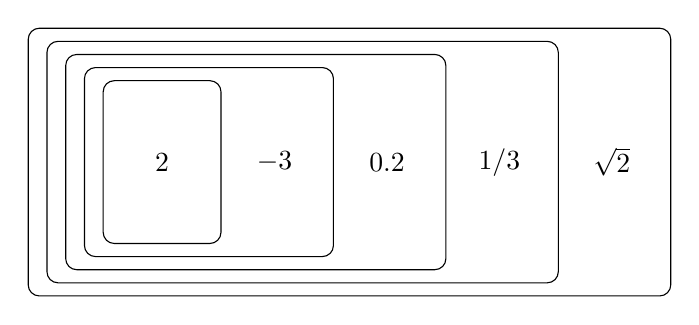
\begin{tikzpicture}[scale=.68]
\foreach \x/\w/\label in {0/12/\R,.35/9.9/\Q,.7/7.8/\D,1.05/5.7/\Z,1.4/3.6/\N}{\draw[rounded corners](\x,\x*.7)rectangle(\w,5-\x*.7);\node at(\w-.35,4.65-\x*.7){$\label$};}
\node at(2.5,2.5){$2$};\node at(4.6,2.5){$-3$};\node at(6.7,2.5){$0.2$};\node at(8.8,2.5){$1/3$};\node at(10.9,2.5){$\sqrt2$};
\end{tikzpicture}\end{center}
\begin{example}Give the smallest of the five sets containing each of the numbers: $-95$; $7.29$; $5/3$; $\sqrt{25}$; $\sqrt2$; $\pi$; $0.0002$.\end{example}
\mxanswerspace[3.2]{$-95\in\Z$; $7.29\in\D$; $5/3\in\Q$; $\sqrt{25}=5\in\N$; $\sqrt2,\pi\in\R\setminus\Q$; $0.0002=2/10^4\in\D$. The irrationality of $\pi$ is accepted here.}

\mxsection{Two proofs by contradiction}
\begin{method}[Proof by contradiction]
To prove a statement, assume its negation, deduce a contradiction, then conclude that the statement is true.
\end{method}
\begin{keypoint}[Property]
$\dfrac13$ is not a decimal number.
\end{keypoint}
\mxwriteproof[5]{Suppose $1/3=a/10^n$ with $a\in\Z$, $n\in\N$. Then $10^n=3a$ would be a multiple of $3$. Yet $10\equiv1$ modulo $3$, so $10^n$ leaves remainder $1$ on division by $3$ (the divisibility rule for $3$ can also be used). Contradiction. Hence $1/3\notin\D$.}
\begin{keypoint}[Property]
$\sqrt2$ is irrational.
\end{keypoint}
\mxwriteproof[6]{Suppose $\sqrt2=p/q$ with $p,q\in\N$, $q\ne0$, and $p/q$ in lowest terms. Then $p^2=2q^2$, so $p^2$ is even. If $p$ were odd, its square would be odd: so $p$ is even. Write $p=2k$. We get $4k^2=2q^2$, then $q^2=2k^2$; so $q$ is even in turn. Thus $2$ divides $p$ and $q$, contradicting irreducibility. Hence $\sqrt2\notin\Q$.}
\begin{teachernote}Have students identify separately the starting hypothesis, the implication used by contraposition on parity, and the final contradiction. Do not present a calculator's decimal expansion as a proof of irrationality.\end{teachernote}

\mxsection{Intervals of the real line}
\begin{keypoint}[Notation]
For two real numbers $a<b$, intervals describe the real numbers lying between two endpoints, with or without the endpoints. A closed bracket includes the endpoint, an open bracket excludes it. The symbols $-\infty,+\infty$ are not real numbers and are always paired with an open bracket.
\end{keypoint}
\begin{center}\mxarraystretch{1.8}\begin{tabular}{c|c|l}
\textbf{Condition}&\textbf{Interval}&\textbf{Description}\\\hline
$a\leq x\leq b$&$[a;b]$&both endpoints included\\
$a<x\leq b$&$]a;b]$&$a$ excluded, $b$ included\\
$a\leq x<b$&$[a;b[$&$a$ included, $b$ excluded\\
$a<x<b$&$]a;b[$&both endpoints excluded\\
$x\geq a$&$[a;+\infty[$&greater than or equal to $a$\\
$x>a$&$]a;+\infty[$&strictly greater than $a$\\
$x\leq b$&$]-\infty;b]$&less than or equal to $b$\\
$x<b$&$]-\infty;b[$&strictly less than $b$
\end{tabular}\end{center}
\[\R=]-\infty;+\infty[,\quad \R^*=]-\infty;0[\,\cup\,]0;+\infty[.\]
\begin{pitfall}The strictly negative real numbers form $]-\infty;0[$: $0$ is excluded. $[a;a]=\{a\}$; $]a;a[=\varnothing$.\end{pitfall}
\begin{example}Write as an interval then represent: $2\leq x\leq5$; $x>4$; $-6<x\leq2$; $x<0$.\end{example}
\mxanswerspace[4]{$[2;5]$; $]4;+\infty[$; $]-6;2]$; $]-\infty;0[$. On the number line, mark the endpoints, then show each one as included or excluded.}

\mxsection{Intersection and union of intervals}
\begin{keypoint}[Definition]
$\,I\cap J$ corresponds to the condition ``belonging to $I$ \textbf{and} to $J$''; $I\cup J$ corresponds to ``belonging to $I$ \textbf{or} to $J$''. A union of intervals is not always an interval.
\end{keypoint}
\begin{example}With $I=[0;12]$ and $J=[3;20]$, determine $I\cap J$ and $I\cup J$.\end{example}
\mxanswerspace[2.4]{$I\cap J=[3;12]$ and $I\cup J=[0;20]$.}
\begin{example}Complete, justifying with representations on a number line.\end{example}
\begin{center}\mxarraystretch{2}\begin{tabular}{c c|c c}
$I$&$J$&$I\cap J$&$I\cup J$\\\hline
$]-4;3]$&$[1;5]$&\mxblank{$[1;3]$}&\mxblank{$]-4;5]$}\\
$]-\infty;2]$&$[-4;+\infty[$&\mxblank{$[-4;2]$}&\mxblank{$\R$}\\
$]-\infty;7]$&$[7;+\infty[$&\mxblank{$\{7\}$}&\mxblank{$\R$}\\
$]-\infty;5]$&$[-3;+\infty[$&\mxblank{$[-3;5]$}&\mxblank{$\R$}\\
$]-2;0[$&$]0;3]$&\mxblank{$\varnothing$}&\mxblank{$]-2;0[\cup]0;3]$}
\end{tabular}\end{center}
\mxanswerspace[4]{For each intersection, keep the points common to both representations; for each union, keep all the points of at least one. In the last row, $0$ belongs to neither interval: the union cannot be replaced by $]-2;3]$.}
\begin{fluency}[5--10 min]Simplify $\vect{AB}+\vect{BC}$; solve $3x-6=0$; calculate $10^{-2}$.\mxanswer{$\vect{AC}$ ; $x=2$ ; $0.01$.}\end{fluency}

\mxsection{Absolute value and distance}
\begin{keypoint}[Definition and properties]
$|x|$ is the distance from the real number $x$ to $0$; $|x|\geq0$ and
\[|x|=\begin{cases}x&\text{if }x\geq0,\\-x&\text{if }x<0.\end{cases}\]
The distance between $a$ and $b$ is $|b-a|$. For $a\in\R$ and $r\geq0$:
\[|x-a|\leq r\iff x\in[a-r;a+r],\qquad |x-a|<r\iff x\in]a-r;a+r[.\]
\end{keypoint}
\begin{example}Calculate $|3.2|$, $|-1.6|$, $|\sqrt3-2|$, then the distances between $2$ and $5$, $2$ and $-5$, $-2$ and $-5$.\end{example}
\mxanswerspace[2.4]{$3.2$; $1.6$; $2-\sqrt3$ since $\sqrt3<2$. The distances are $3$, $7$ and $3$.}
\begin{example}Solve: $|x-7/3|=14$; $|x-2|\leq3$; $|x+3|<5$.\end{example}
\mxanswerspace[4.8]{For the first equation, $x-7/3=14$ or $x-7/3=-14$, so $S=\{-35/3;49/3\}$. Then $|x-2|\leq3\iff x\in[-1;5]$. Finally $|x+3|=|x-(-3)|<5\iff x\in]-8;2[$.}
\begin{example}Write $x\in[4;10]$ as an inequality with an absolute value.\end{example}
\mxanswerspace[2]{The centre is $(4+10)/2=7$ and the radius $(10-4)/2=3$: $|x-7|\leq3$.}

\mxsection{Bounds and approximations}
\begin{keypoint}[Vocabulary]
To bound $x$ is to give $a\leq x\leq b$; the width is $b-a$. An approximation from below is less than or equal to $x$; an approximation from above is greater than or equal to it. Rounding chooses the nearest value at the required precision.
Significant figures are counted from the first nonzero digit; the displayed precision must suit the context.
\end{keypoint}
\begin{example}Bound $\sqrt2$ between two consecutive hundredths. Give its rounding to the nearest hundredth. Round $0.004567$ to three significant figures, then $12345$ to three significant figures in scientific notation.\end{example}
\mxanswerspace[3.2]{$1.41^2=1.9881<2<2.0164=1.42^2$, so $1.41<\sqrt2<1.42$ (width $0.01$). The rounding to the nearest hundredth is $1.41$. The other roundings are $0.00457$ and $1.23\times10^4$.}
\begin{lstlisting}
def encadre_racine2(p):
    # p entier naturel ; calculs entiers exacts
    q = 10**p
    k = 0
    while (k+1)**2 <= 2*q*q:
        k = k+1
    return k/q, (k+1)/q
\end{lstlisting}
\begin{example}Explain why this function bounds $\sqrt2$. What does it return for $p=2$? Why does it terminate?\end{example}
\mxanswerspace[3.2]{The loop looks for the largest integer $k$ such that $k^2\leq2q^2$. On exit, $k^2\leq2q^2<(k+1)^2$, so $k/q\leq\sqrt2<(k+1)/q$. For $p=2$, it returns $(1.41;1.42)$. Since $(2q)^2>2q^2$, the counter eventually reaches a value that makes the test false. The final divisions are floating-point approximations; the square tests are exact.}
